\documentclass[twoside]{book}

% Packages required by doxygen
\usepackage{fixltx2e}
\usepackage{calc}
\usepackage{doxygen}
\usepackage[export]{adjustbox} % also loads graphicx
\usepackage{graphicx}
\usepackage[utf8]{inputenc}
\usepackage{makeidx}
\usepackage{multicol}
\usepackage{multirow}
\PassOptionsToPackage{warn}{textcomp}
\usepackage{textcomp}
\usepackage[nointegrals]{wasysym}
\usepackage[table]{xcolor}

% NLS support packages
\usepackage[spanish]{babel}
% Font selection
\usepackage[T1]{fontenc}
\usepackage[scaled=.90]{helvet}
\usepackage{courier}
\usepackage{amssymb}
\usepackage{sectsty}
\renewcommand{\familydefault}{\sfdefault}
\allsectionsfont{%
  \fontseries{bc}\selectfont%
  \color{darkgray}%
}
\renewcommand{\DoxyLabelFont}{%
  \fontseries{bc}\selectfont%
  \color{darkgray}%
}
\newcommand{\+}{\discretionary{\mbox{\scriptsize$\hookleftarrow$}}{}{}}

% Page & text layout
\usepackage{geometry}
\geometry{%
  a4paper,%
  top=2.5cm,%
  bottom=2.5cm,%
  left=2.5cm,%
  right=2.5cm%
}
\tolerance=750
\hfuzz=15pt
\hbadness=750
\setlength{\emergencystretch}{15pt}
\setlength{\parindent}{0cm}
\setlength{\parskip}{3ex plus 2ex minus 2ex}
\makeatletter
\renewcommand{\paragraph}{%
  \@startsection{paragraph}{4}{0ex}{-1.0ex}{1.0ex}{%
    \normalfont\normalsize\bfseries\SS@parafont%
  }%
}
\renewcommand{\subparagraph}{%
  \@startsection{subparagraph}{5}{0ex}{-1.0ex}{1.0ex}{%
    \normalfont\normalsize\bfseries\SS@subparafont%
  }%
}
\makeatother

% Headers & footers
\usepackage{fancyhdr}
\pagestyle{fancyplain}
\fancyhead[LE]{\fancyplain{}{\bfseries\thepage}}
\fancyhead[CE]{\fancyplain{}{}}
\fancyhead[RE]{\fancyplain{}{\bfseries\leftmark}}
\fancyhead[LO]{\fancyplain{}{\bfseries\rightmark}}
\fancyhead[CO]{\fancyplain{}{}}
\fancyhead[RO]{\fancyplain{}{\bfseries\thepage}}
\fancyfoot[LE]{\fancyplain{}{}}
\fancyfoot[CE]{\fancyplain{}{}}
\fancyfoot[RE]{\fancyplain{}{\bfseries\scriptsize Generado por Doxygen }}
\fancyfoot[LO]{\fancyplain{}{\bfseries\scriptsize Generado por Doxygen }}
\fancyfoot[CO]{\fancyplain{}{}}
\fancyfoot[RO]{\fancyplain{}{}}
\renewcommand{\footrulewidth}{0.4pt}
\renewcommand{\chaptermark}[1]{%
  \markboth{#1}{}%
}
\renewcommand{\sectionmark}[1]{%
  \markright{\thesection\ #1}%
}

% Indices & bibliography
\usepackage{natbib}
\usepackage[titles]{tocloft}
\setcounter{tocdepth}{3}
\setcounter{secnumdepth}{5}
\makeindex

% Hyperlinks (required, but should be loaded last)
\usepackage{ifpdf}
\ifpdf
  \usepackage[pdftex,pagebackref=true]{hyperref}
\else
  \usepackage[ps2pdf,pagebackref=true]{hyperref}
\fi
\hypersetup{%
  colorlinks=true,%
  linkcolor=blue,%
  citecolor=blue,%
  unicode%
}

% Custom commands
\newcommand{\clearemptydoublepage}{%
  \newpage{\pagestyle{empty}\cleardoublepage}%
}

\usepackage{caption}
\captionsetup{labelsep=space,justification=centering,font={bf},singlelinecheck=off,skip=4pt,position=top}

%===== C O N T E N T S =====

\begin{document}

% Titlepage & ToC
\hypersetup{pageanchor=false,
             bookmarksnumbered=true,
             pdfencoding=unicode
            }
\pagenumbering{alph}
\begin{titlepage}
\vspace*{7cm}
\begin{center}%
{\Large Pràctica P\+R\+O2 -\/ Ferran Mateu \\[1ex]\large Inici\+: 12 abril 2019, Final\+: }\\
\vspace*{1cm}
{\large Generado por Doxygen 1.8.13}\\
\end{center}
\end{titlepage}
\clearemptydoublepage
\pagenumbering{roman}
\tableofcontents
\clearemptydoublepage
\pagenumbering{arabic}
\hypersetup{pageanchor=true}

%--- Begin generated contents ---
\chapter{Gestió de la codificació i la decodificació en funció de diferent idiomes.}
\label{index}\hypertarget{index}{}En aquesta pàgina hi ha l\textquotesingle{}especificació de la pràctica de P\+R\+O2 de 2019.

En ella apareixen els arxius on s\textquotesingle{}especifiquen les funcions que fa servir el programa principal \hyperlink{program_8cc}{program.\+cc} 
\chapter{Índice de clases}
\section{Lista de clases}
Lista de las clases, estructuras, uniones e interfaces con una breve descripción\+:\begin{DoxyCompactList}
\item\contentsline{section}{\hyperlink{class_cjt___idiomes}{Cjt\+\_\+\+Idiomes} \\*Representa un \hyperlink{class_cjt___idiomes}{Cjt\+\_\+\+Idiomes} }{\pageref{class_cjt___idiomes}}{}
\item\contentsline{section}{\hyperlink{structcomp}{comp} }{\pageref{structcomp}}{}
\item\contentsline{section}{\hyperlink{class_idioma}{Idioma} \\*Representa un \hyperlink{class_idioma}{Idioma} }{\pageref{class_idioma}}{}
\item\contentsline{section}{\hyperlink{class_taula__de__freq}{Taula\+\_\+de\+\_\+freq} \\*Representa una \hyperlink{class_taula__de__freq}{Taula\+\_\+de\+\_\+freq} }{\pageref{class_taula__de__freq}}{}
\item\contentsline{section}{\hyperlink{class_treecode}{Treecode} \\*Representa una \hyperlink{class_treecode}{Treecode} }{\pageref{class_treecode}}{}
\end{DoxyCompactList}

\chapter{Indice de archivos}
\section{Lista de archivos}
Lista de todos los archivos con descripciones breves\+:\begin{DoxyCompactList}
\item\contentsline{section}{\hyperlink{_cjt___idiomes_8hh}{Cjt\+\_\+\+Idiomes.\+hh} \\*Especificació de la classe \hyperlink{class_cjt___idiomes}{Cjt\+\_\+\+Idiomes} }{\pageref{_cjt___idiomes_8hh}}{}
\item\contentsline{section}{\hyperlink{_idioma_8hh}{Idioma.\+hh} \\*Especificació de la classe \hyperlink{class_idioma}{Idioma} }{\pageref{_idioma_8hh}}{}
\item\contentsline{section}{\hyperlink{program_8cc}{program.\+cc} \\*Programa principal per la gestió de codificar i descodificar }{\pageref{program_8cc}}{}
\item\contentsline{section}{\hyperlink{_taula__de__codis_8hh}{Taula\+\_\+de\+\_\+codis.\+hh} \\*Especificació de la classe \hyperlink{class_taula__de__codis}{Taula\+\_\+de\+\_\+codis} }{\pageref{_taula__de__codis_8hh}}{}
\item\contentsline{section}{\hyperlink{_taula__de__freq_8hh}{Taula\+\_\+de\+\_\+freq.\+hh} \\*Especificació de la classe \hyperlink{class_taula__de__freq}{Taula\+\_\+de\+\_\+freq} }{\pageref{_taula__de__freq_8hh}}{}
\item\contentsline{section}{\hyperlink{_treecode_8hh}{Treecode.\+hh} \\*Especificació de la classe \hyperlink{class_treecode}{Treecode} }{\pageref{_treecode_8hh}}{}
\end{DoxyCompactList}

\chapter{Documentación de las clases}
\hypertarget{class_cjt___idiomes}{}\section{Referencia de la Clase Cjt\+\_\+\+Idiomes}
\label{class_cjt___idiomes}\index{Cjt\+\_\+\+Idiomes@{Cjt\+\_\+\+Idiomes}}


Representa un \hyperlink{class_cjt___idiomes}{Cjt\+\_\+\+Idiomes}.  


\subsection*{Métodos públicos}
\begin{DoxyCompactItemize}
\item 
\hyperlink{class_cjt___idiomes_af77cbc534e3e83142a818314f5c24ae3}{Cjt\+\_\+\+Idiomes} ()
\begin{DoxyCompactList}\small\item\em Crea un conjunt d\textquotesingle{}idiomes buit. \end{DoxyCompactList}\item 
\hyperlink{class_cjt___idiomes_ab36517bd1824e0f00cab6cf724b6ad6f}{$\sim$\+Cjt\+\_\+\+Idiomes} ()
\item 
void \hyperlink{class_cjt___idiomes_a27ad0dd99449fffa904e6a757b4388ad}{omplir\+\_\+cjt\+\_\+idiomes} ()
\begin{DoxyCompactList}\small\item\em Omple un conjunt d\textquotesingle{}idiomes amb n idiomes. \end{DoxyCompactList}\item 
void \hyperlink{class_cjt___idiomes_a9e75f643c62886df635403bd3108c1df}{afegir\+\_\+modificar\+\_\+idioma} (const string \&idioma)
\begin{DoxyCompactList}\small\item\em Afegeix un idioma o el modifica. \end{DoxyCompactList}\item 
string \hyperlink{class_cjt___idiomes_a745de8e5d29e235cb1e2142d8acaaad9}{codifica} (string idioma, string \&text)
\begin{DoxyCompactList}\small\item\em Codifica un text en un idioma. \end{DoxyCompactList}\item 
string \hyperlink{class_cjt___idiomes_ab77062c4c2b311bbc1fc1143073bc036}{decodifica} (string idioma, string \&text)
\begin{DoxyCompactList}\small\item\em Decodifica un text en un idioma. \end{DoxyCompactList}\item 
void \hyperlink{class_cjt___idiomes_af0cfe6e69c1784af172fe825bdbe61f8}{consultar\+\_\+taula\+\_\+freq} (string idioma)
\begin{DoxyCompactList}\small\item\em Consulta la taula de freq del idioma en el paràmetre implícit. \end{DoxyCompactList}\item 
bool \hyperlink{class_cjt___idiomes_a4c46be5ecf3b12b3f481ace7d487fdc3}{idioma\+\_\+esta} (string idioma)
\begin{DoxyCompactList}\small\item\em Comprva si un idioma es troba al conjunt o no. \end{DoxyCompactList}\item 
void \hyperlink{class_cjt___idiomes_a7aad6974355b73c50c2d5c1edc0a5c14}{actualitza\+\_\+idioma} (string nomidioma)
\begin{DoxyCompactList}\small\item\em Actualitza el treecode, la taula de codis i la taula de freqüències del idioma passat com a paràmetre. \end{DoxyCompactList}\item 
void \hyperlink{class_cjt___idiomes_a49666adf7e2a9cefc96d4b7b3d925710}{escriure\+\_\+treecode} (string nomidioma)
\begin{DoxyCompactList}\small\item\em Escriu el treecode del paràmetre implícit. \end{DoxyCompactList}\item 
void \hyperlink{class_cjt___idiomes_afdad5e96949152abf75a9598224be426}{escriure\+\_\+taulacodis} (string nomidioma, string s)
\begin{DoxyCompactList}\small\item\em Escriu la taula de codis del paràmetre implícit. \end{DoxyCompactList}\item 
void \hyperlink{class_cjt___idiomes_a98862ab41b59ac71eca4408e2b6bf6f0}{escriure\+\_\+taulafreq} (string nomidioma)
\begin{DoxyCompactList}\small\item\em Escriu la taula de freqüències del paràmetre implícit. \end{DoxyCompactList}\end{DoxyCompactItemize}


\subsection{Descripción detallada}
Representa un \hyperlink{class_cjt___idiomes}{Cjt\+\_\+\+Idiomes}. 

Definición en la línea 17 del archivo Cjt\+\_\+\+Idiomes.\+hh.



\subsection{Documentación del constructor y destructor}
\mbox{\Hypertarget{class_cjt___idiomes_af77cbc534e3e83142a818314f5c24ae3}\label{class_cjt___idiomes_af77cbc534e3e83142a818314f5c24ae3}} 
\index{Cjt\+\_\+\+Idiomes@{Cjt\+\_\+\+Idiomes}!Cjt\+\_\+\+Idiomes@{Cjt\+\_\+\+Idiomes}}
\index{Cjt\+\_\+\+Idiomes@{Cjt\+\_\+\+Idiomes}!Cjt\+\_\+\+Idiomes@{Cjt\+\_\+\+Idiomes}}
\subsubsection{\texorpdfstring{Cjt\+\_\+\+Idiomes()}{Cjt\_Idiomes()}}
{\footnotesize\ttfamily Cjt\+\_\+\+Idiomes\+::\+Cjt\+\_\+\+Idiomes (\begin{DoxyParamCaption}{ }\end{DoxyParamCaption})}



Crea un conjunt d\textquotesingle{}idiomes buit. 

\begin{DoxyPrecond}{Precondición}
{\itshape Cert} 
\end{DoxyPrecond}
\begin{DoxyPostcond}{Postcondición}
S\textquotesingle{}ha creat un conjunt d\textquotesingle{}idiomes buit 
\end{DoxyPostcond}
\mbox{\Hypertarget{class_cjt___idiomes_ab36517bd1824e0f00cab6cf724b6ad6f}\label{class_cjt___idiomes_ab36517bd1824e0f00cab6cf724b6ad6f}} 
\index{Cjt\+\_\+\+Idiomes@{Cjt\+\_\+\+Idiomes}!````~Cjt\+\_\+\+Idiomes@{$\sim$\+Cjt\+\_\+\+Idiomes}}
\index{````~Cjt\+\_\+\+Idiomes@{$\sim$\+Cjt\+\_\+\+Idiomes}!Cjt\+\_\+\+Idiomes@{Cjt\+\_\+\+Idiomes}}
\subsubsection{\texorpdfstring{$\sim$\+Cjt\+\_\+\+Idiomes()}{~Cjt\_Idiomes()}}
{\footnotesize\ttfamily Cjt\+\_\+\+Idiomes\+::$\sim$\+Cjt\+\_\+\+Idiomes (\begin{DoxyParamCaption}{ }\end{DoxyParamCaption})}



\subsection{Documentación de las funciones miembro}
\mbox{\Hypertarget{class_cjt___idiomes_a27ad0dd99449fffa904e6a757b4388ad}\label{class_cjt___idiomes_a27ad0dd99449fffa904e6a757b4388ad}} 
\index{Cjt\+\_\+\+Idiomes@{Cjt\+\_\+\+Idiomes}!omplir\+\_\+cjt\+\_\+idiomes@{omplir\+\_\+cjt\+\_\+idiomes}}
\index{omplir\+\_\+cjt\+\_\+idiomes@{omplir\+\_\+cjt\+\_\+idiomes}!Cjt\+\_\+\+Idiomes@{Cjt\+\_\+\+Idiomes}}
\subsubsection{\texorpdfstring{omplir\+\_\+cjt\+\_\+idiomes()}{omplir\_cjt\_idiomes()}}
{\footnotesize\ttfamily void Cjt\+\_\+\+Idiomes\+::omplir\+\_\+cjt\+\_\+idiomes (\begin{DoxyParamCaption}{ }\end{DoxyParamCaption})}



Omple un conjunt d\textquotesingle{}idiomes amb n idiomes. 

\begin{DoxyPrecond}{Precondición}
Conj buit, n$>$=0, llista d\textquotesingle{}idiomes en el canal d\textquotesingle{}entrada 
\end{DoxyPrecond}
\begin{DoxyPostcond}{Postcondición}
El conjunt d\textquotesingle{}idiomes ha quedat ple amb els n idiomes del canal d\textquotesingle{}entrada 
\end{DoxyPostcond}
\mbox{\Hypertarget{class_cjt___idiomes_a9e75f643c62886df635403bd3108c1df}\label{class_cjt___idiomes_a9e75f643c62886df635403bd3108c1df}} 
\index{Cjt\+\_\+\+Idiomes@{Cjt\+\_\+\+Idiomes}!afegir\+\_\+modificar\+\_\+idioma@{afegir\+\_\+modificar\+\_\+idioma}}
\index{afegir\+\_\+modificar\+\_\+idioma@{afegir\+\_\+modificar\+\_\+idioma}!Cjt\+\_\+\+Idiomes@{Cjt\+\_\+\+Idiomes}}
\subsubsection{\texorpdfstring{afegir\+\_\+modificar\+\_\+idioma()}{afegir\_modificar\_idioma()}}
{\footnotesize\ttfamily void Cjt\+\_\+\+Idiomes\+::afegir\+\_\+modificar\+\_\+idioma (\begin{DoxyParamCaption}\item[{const string \&}]{idioma }\end{DoxyParamCaption})}



Afegeix un idioma o el modifica. 

\begin{DoxyPrecond}{Precondición}
{\itshape cert} 
\end{DoxyPrecond}
\begin{DoxyPostcond}{Postcondición}
El paràmetre implícit s\textquotesingle{}hi ha afegit l\textquotesingle{}idioma si no hi era, sinó, s\textquotesingle{}ha modificat l\textquotesingle{}idioma sumant les freqüències. 
\end{DoxyPostcond}
\mbox{\Hypertarget{class_cjt___idiomes_a745de8e5d29e235cb1e2142d8acaaad9}\label{class_cjt___idiomes_a745de8e5d29e235cb1e2142d8acaaad9}} 
\index{Cjt\+\_\+\+Idiomes@{Cjt\+\_\+\+Idiomes}!codifica@{codifica}}
\index{codifica@{codifica}!Cjt\+\_\+\+Idiomes@{Cjt\+\_\+\+Idiomes}}
\subsubsection{\texorpdfstring{codifica()}{codifica()}}
{\footnotesize\ttfamily string Cjt\+\_\+\+Idiomes\+::codifica (\begin{DoxyParamCaption}\item[{string}]{idioma,  }\item[{string \&}]{text }\end{DoxyParamCaption})}



Codifica un text en un idioma. 

\begin{DoxyPrecond}{Precondición}
L\textquotesingle{}idioma es troba al conjunt 
\end{DoxyPrecond}
\begin{DoxyPostcond}{Postcondición}
Si el text es pot codificar, retorna un string amb el text codificat, sinó, informa de que no el text no pertany a l\textquotesingle{}idioma 
\end{DoxyPostcond}
\mbox{\Hypertarget{class_cjt___idiomes_ab77062c4c2b311bbc1fc1143073bc036}\label{class_cjt___idiomes_ab77062c4c2b311bbc1fc1143073bc036}} 
\index{Cjt\+\_\+\+Idiomes@{Cjt\+\_\+\+Idiomes}!decodifica@{decodifica}}
\index{decodifica@{decodifica}!Cjt\+\_\+\+Idiomes@{Cjt\+\_\+\+Idiomes}}
\subsubsection{\texorpdfstring{decodifica()}{decodifica()}}
{\footnotesize\ttfamily string Cjt\+\_\+\+Idiomes\+::decodifica (\begin{DoxyParamCaption}\item[{string}]{idioma,  }\item[{string \&}]{text }\end{DoxyParamCaption})}



Decodifica un text en un idioma. 

\begin{DoxyPrecond}{Precondición}
L\textquotesingle{}idioma es troba al conjunt 
\end{DoxyPrecond}
\begin{DoxyPostcond}{Postcondición}
Si el text codificat pertany a l\textquotesingle{}idioma, retorna un string amb el text de codificat, sinó, informa de que no el text no pertany a l\textquotesingle{}idioma 
\end{DoxyPostcond}
\mbox{\Hypertarget{class_cjt___idiomes_af0cfe6e69c1784af172fe825bdbe61f8}\label{class_cjt___idiomes_af0cfe6e69c1784af172fe825bdbe61f8}} 
\index{Cjt\+\_\+\+Idiomes@{Cjt\+\_\+\+Idiomes}!consultar\+\_\+taula\+\_\+freq@{consultar\+\_\+taula\+\_\+freq}}
\index{consultar\+\_\+taula\+\_\+freq@{consultar\+\_\+taula\+\_\+freq}!Cjt\+\_\+\+Idiomes@{Cjt\+\_\+\+Idiomes}}
\subsubsection{\texorpdfstring{consultar\+\_\+taula\+\_\+freq()}{consultar\_taula\_freq()}}
{\footnotesize\ttfamily void Cjt\+\_\+\+Idiomes\+::consultar\+\_\+taula\+\_\+freq (\begin{DoxyParamCaption}\item[{string}]{idioma }\end{DoxyParamCaption})}



Consulta la taula de freq del idioma en el paràmetre implícit. 

\begin{DoxyPrecond}{Precondición}
L\textquotesingle{}idioma es troba al conjunt 
\end{DoxyPrecond}
\begin{DoxyPostcond}{Postcondición}
Retorna la taula de freq del idioma especificat 
\end{DoxyPostcond}
\mbox{\Hypertarget{class_cjt___idiomes_a4c46be5ecf3b12b3f481ace7d487fdc3}\label{class_cjt___idiomes_a4c46be5ecf3b12b3f481ace7d487fdc3}} 
\index{Cjt\+\_\+\+Idiomes@{Cjt\+\_\+\+Idiomes}!idioma\+\_\+esta@{idioma\+\_\+esta}}
\index{idioma\+\_\+esta@{idioma\+\_\+esta}!Cjt\+\_\+\+Idiomes@{Cjt\+\_\+\+Idiomes}}
\subsubsection{\texorpdfstring{idioma\+\_\+esta()}{idioma\_esta()}}
{\footnotesize\ttfamily bool Cjt\+\_\+\+Idiomes\+::idioma\+\_\+esta (\begin{DoxyParamCaption}\item[{string}]{idioma }\end{DoxyParamCaption})}



Comprva si un idioma es troba al conjunt o no. 

\begin{DoxyPrecond}{Precondición}
{\itshape Cert} 
\end{DoxyPrecond}
\begin{DoxyPostcond}{Postcondición}
Retorna un boleà en funció de si l\textquotesingle{}idioma es troba al paràmetre implícit o no 
\end{DoxyPostcond}
\mbox{\Hypertarget{class_cjt___idiomes_a7aad6974355b73c50c2d5c1edc0a5c14}\label{class_cjt___idiomes_a7aad6974355b73c50c2d5c1edc0a5c14}} 
\index{Cjt\+\_\+\+Idiomes@{Cjt\+\_\+\+Idiomes}!actualitza\+\_\+idioma@{actualitza\+\_\+idioma}}
\index{actualitza\+\_\+idioma@{actualitza\+\_\+idioma}!Cjt\+\_\+\+Idiomes@{Cjt\+\_\+\+Idiomes}}
\subsubsection{\texorpdfstring{actualitza\+\_\+idioma()}{actualitza\_idioma()}}
{\footnotesize\ttfamily void Cjt\+\_\+\+Idiomes\+::actualitza\+\_\+idioma (\begin{DoxyParamCaption}\item[{string}]{nomidioma }\end{DoxyParamCaption})}



Actualitza el treecode, la taula de codis i la taula de freqüències del idioma passat com a paràmetre. 

\begin{DoxyPrecond}{Precondición}
{\itshape Cert} 
\end{DoxyPrecond}
\begin{DoxyPostcond}{Postcondición}
L\textquotesingle{}idioma ha quedat actualitzat amb les noves freqüències i codis. 
\end{DoxyPostcond}
\mbox{\Hypertarget{class_cjt___idiomes_a49666adf7e2a9cefc96d4b7b3d925710}\label{class_cjt___idiomes_a49666adf7e2a9cefc96d4b7b3d925710}} 
\index{Cjt\+\_\+\+Idiomes@{Cjt\+\_\+\+Idiomes}!escriure\+\_\+treecode@{escriure\+\_\+treecode}}
\index{escriure\+\_\+treecode@{escriure\+\_\+treecode}!Cjt\+\_\+\+Idiomes@{Cjt\+\_\+\+Idiomes}}
\subsubsection{\texorpdfstring{escriure\+\_\+treecode()}{escriure\_treecode()}}
{\footnotesize\ttfamily void Cjt\+\_\+\+Idiomes\+::escriure\+\_\+treecode (\begin{DoxyParamCaption}\item[{string}]{nomidioma }\end{DoxyParamCaption})}



Escriu el treecode del paràmetre implícit. 

\begin{DoxyPrecond}{Precondición}
{\itshape Cert} 
\end{DoxyPrecond}
\begin{DoxyPostcond}{Postcondición}
S\textquotesingle{}ha escrit el treecode pel canal estàndard de sortida 
\end{DoxyPostcond}
\mbox{\Hypertarget{class_cjt___idiomes_afdad5e96949152abf75a9598224be426}\label{class_cjt___idiomes_afdad5e96949152abf75a9598224be426}} 
\index{Cjt\+\_\+\+Idiomes@{Cjt\+\_\+\+Idiomes}!escriure\+\_\+taulacodis@{escriure\+\_\+taulacodis}}
\index{escriure\+\_\+taulacodis@{escriure\+\_\+taulacodis}!Cjt\+\_\+\+Idiomes@{Cjt\+\_\+\+Idiomes}}
\subsubsection{\texorpdfstring{escriure\+\_\+taulacodis()}{escriure\_taulacodis()}}
{\footnotesize\ttfamily void Cjt\+\_\+\+Idiomes\+::escriure\+\_\+taulacodis (\begin{DoxyParamCaption}\item[{string}]{nomidioma,  }\item[{string}]{s }\end{DoxyParamCaption})}



Escriu la taula de codis del paràmetre implícit. 

\begin{DoxyPrecond}{Precondición}
{\itshape Cert} 
\end{DoxyPrecond}
\begin{DoxyPostcond}{Postcondición}
S\textquotesingle{}ha escrit la taula de codis pel canal estàndard de sortida 
\end{DoxyPostcond}
\mbox{\Hypertarget{class_cjt___idiomes_a98862ab41b59ac71eca4408e2b6bf6f0}\label{class_cjt___idiomes_a98862ab41b59ac71eca4408e2b6bf6f0}} 
\index{Cjt\+\_\+\+Idiomes@{Cjt\+\_\+\+Idiomes}!escriure\+\_\+taulafreq@{escriure\+\_\+taulafreq}}
\index{escriure\+\_\+taulafreq@{escriure\+\_\+taulafreq}!Cjt\+\_\+\+Idiomes@{Cjt\+\_\+\+Idiomes}}
\subsubsection{\texorpdfstring{escriure\+\_\+taulafreq()}{escriure\_taulafreq()}}
{\footnotesize\ttfamily void Cjt\+\_\+\+Idiomes\+::escriure\+\_\+taulafreq (\begin{DoxyParamCaption}\item[{string}]{nomidioma }\end{DoxyParamCaption})}



Escriu la taula de freqüències del paràmetre implícit. 

\begin{DoxyPrecond}{Precondición}
{\itshape Cert} 
\end{DoxyPrecond}
\begin{DoxyPostcond}{Postcondición}
S\textquotesingle{}ha escrit la taula de freqüències pel canal estàndard de sortida 
\end{DoxyPostcond}


La documentación para esta clase fue generada a partir del siguiente fichero\+:\begin{DoxyCompactItemize}
\item 
\hyperlink{_cjt___idiomes_8hh}{Cjt\+\_\+\+Idiomes.\+hh}\end{DoxyCompactItemize}

\hypertarget{class_idioma}{}\section{Referencia de la Clase Idioma}
\label{class_idioma}\index{Idioma@{Idioma}}


Representa un \hyperlink{class_idioma}{Idioma}.  


\subsection*{Métodos públicos}
\begin{DoxyCompactItemize}
\item 
\hyperlink{class_idioma_acb367feda82c466b5c61378636b901b6}{Idioma} (string nom)
\begin{DoxyCompactList}\small\item\em Crea un \hyperlink{class_idioma}{Idioma} amb el seu nom. \end{DoxyCompactList}\item 
\hyperlink{class_idioma_a80c90f8c9a7f824d7d7d171b9face201}{$\sim$\+Idioma} ()
\item 
void \hyperlink{class_idioma_afcdc214d9490b61d54e35da85f2354a4}{actualitza\+\_\+treecode} ()
\begin{DoxyCompactList}\small\item\em Actualitza el treecode de l\textquotesingle{}idioma del paràmetre implícit. \end{DoxyCompactList}\item 
void \hyperlink{class_idioma_ac089a0e4b79ca8f3df040e204a3de7dd}{actualitza\+\_\+taulacodis} ()
\begin{DoxyCompactList}\small\item\em Actualitza la taula de codis de l\textquotesingle{}idioma del paràmetre implícit. \end{DoxyCompactList}\item 
\hyperlink{class_taula__de__freq}{Taula\+\_\+de\+\_\+freq} \hyperlink{class_idioma_a3d06a9d14291a5b59e0de1a65512ed80}{consultar\+\_\+taula\+\_\+freq} ()
\begin{DoxyCompactList}\small\item\em Consulta la taula de freqüències de l\textquotesingle{}idioma del paràmetre implícit. \end{DoxyCompactList}\item 
void \hyperlink{class_idioma_a2c3024b18da125926668a2df2b178992}{escriure\+\_\+treecode} ()
\begin{DoxyCompactList}\small\item\em Escriu el treecode de l\textquotesingle{}idioma del paràmetre implícit. \end{DoxyCompactList}\item 
void \hyperlink{class_idioma_a4f1102ff409d13738ff09268e8e045da}{escriure\+\_\+taulacodis} (string s)
\begin{DoxyCompactList}\small\item\em Escriu la taula de codis de l\textquotesingle{}idioma del paràmetre implícit. \end{DoxyCompactList}\end{DoxyCompactItemize}


\subsection{Descripción detallada}
Representa un \hyperlink{class_idioma}{Idioma}. 

Definición en la línea 20 del archivo Idioma.\+hh.



\subsection{Documentación del constructor y destructor}
\mbox{\Hypertarget{class_idioma_acb367feda82c466b5c61378636b901b6}\label{class_idioma_acb367feda82c466b5c61378636b901b6}} 
\index{Idioma@{Idioma}!Idioma@{Idioma}}
\index{Idioma@{Idioma}!Idioma@{Idioma}}
\subsubsection{\texorpdfstring{Idioma()}{Idioma()}}
{\footnotesize\ttfamily Idioma\+::\+Idioma (\begin{DoxyParamCaption}\item[{string}]{nom }\end{DoxyParamCaption})}



Crea un \hyperlink{class_idioma}{Idioma} amb el seu nom. 

\begin{DoxyPrecond}{Precondición}
{\itshape cert} 
\end{DoxyPrecond}
\begin{DoxyPostcond}{Postcondición}
S\textquotesingle{}ha creat un idioma amb el nom. 
\end{DoxyPostcond}
\mbox{\Hypertarget{class_idioma_a80c90f8c9a7f824d7d7d171b9face201}\label{class_idioma_a80c90f8c9a7f824d7d7d171b9face201}} 
\index{Idioma@{Idioma}!````~Idioma@{$\sim$\+Idioma}}
\index{````~Idioma@{$\sim$\+Idioma}!Idioma@{Idioma}}
\subsubsection{\texorpdfstring{$\sim$\+Idioma()}{~Idioma()}}
{\footnotesize\ttfamily Idioma\+::$\sim$\+Idioma (\begin{DoxyParamCaption}{ }\end{DoxyParamCaption})}



\subsection{Documentación de las funciones miembro}
\mbox{\Hypertarget{class_idioma_afcdc214d9490b61d54e35da85f2354a4}\label{class_idioma_afcdc214d9490b61d54e35da85f2354a4}} 
\index{Idioma@{Idioma}!actualitza\+\_\+treecode@{actualitza\+\_\+treecode}}
\index{actualitza\+\_\+treecode@{actualitza\+\_\+treecode}!Idioma@{Idioma}}
\subsubsection{\texorpdfstring{actualitza\+\_\+treecode()}{actualitza\_treecode()}}
{\footnotesize\ttfamily void Idioma\+::actualitza\+\_\+treecode (\begin{DoxyParamCaption}{ }\end{DoxyParamCaption})}



Actualitza el treecode de l\textquotesingle{}idioma del paràmetre implícit. 

\begin{DoxyPrecond}{Precondición}
{\itshape cert} 
\end{DoxyPrecond}
\begin{DoxyPostcond}{Postcondición}
S\textquotesingle{}ha actualitzat el treecode del paràmetre implícit 
\end{DoxyPostcond}
\mbox{\Hypertarget{class_idioma_ac089a0e4b79ca8f3df040e204a3de7dd}\label{class_idioma_ac089a0e4b79ca8f3df040e204a3de7dd}} 
\index{Idioma@{Idioma}!actualitza\+\_\+taulacodis@{actualitza\+\_\+taulacodis}}
\index{actualitza\+\_\+taulacodis@{actualitza\+\_\+taulacodis}!Idioma@{Idioma}}
\subsubsection{\texorpdfstring{actualitza\+\_\+taulacodis()}{actualitza\_taulacodis()}}
{\footnotesize\ttfamily void Idioma\+::actualitza\+\_\+taulacodis (\begin{DoxyParamCaption}{ }\end{DoxyParamCaption})}



Actualitza la taula de codis de l\textquotesingle{}idioma del paràmetre implícit. 

\begin{DoxyPrecond}{Precondición}
{\itshape cert} 
\end{DoxyPrecond}
\begin{DoxyPostcond}{Postcondición}
S\textquotesingle{}ha actualitzat la taula de codis del paràmetre implícit 
\end{DoxyPostcond}
\mbox{\Hypertarget{class_idioma_a3d06a9d14291a5b59e0de1a65512ed80}\label{class_idioma_a3d06a9d14291a5b59e0de1a65512ed80}} 
\index{Idioma@{Idioma}!consultar\+\_\+taula\+\_\+freq@{consultar\+\_\+taula\+\_\+freq}}
\index{consultar\+\_\+taula\+\_\+freq@{consultar\+\_\+taula\+\_\+freq}!Idioma@{Idioma}}
\subsubsection{\texorpdfstring{consultar\+\_\+taula\+\_\+freq()}{consultar\_taula\_freq()}}
{\footnotesize\ttfamily \hyperlink{class_taula__de__freq}{Taula\+\_\+de\+\_\+freq} Idioma\+::consultar\+\_\+taula\+\_\+freq (\begin{DoxyParamCaption}{ }\end{DoxyParamCaption})}



Consulta la taula de freqüències de l\textquotesingle{}idioma del paràmetre implícit. 

\begin{DoxyPrecond}{Precondición}
{\itshape cert} 
\end{DoxyPrecond}
\begin{DoxyPostcond}{Postcondición}
Retorna la taula de freqüències del paràmetre implícit 
\end{DoxyPostcond}
\mbox{\Hypertarget{class_idioma_a2c3024b18da125926668a2df2b178992}\label{class_idioma_a2c3024b18da125926668a2df2b178992}} 
\index{Idioma@{Idioma}!escriure\+\_\+treecode@{escriure\+\_\+treecode}}
\index{escriure\+\_\+treecode@{escriure\+\_\+treecode}!Idioma@{Idioma}}
\subsubsection{\texorpdfstring{escriure\+\_\+treecode()}{escriure\_treecode()}}
{\footnotesize\ttfamily void Idioma\+::escriure\+\_\+treecode (\begin{DoxyParamCaption}{ }\end{DoxyParamCaption})}



Escriu el treecode de l\textquotesingle{}idioma del paràmetre implícit. 

\begin{DoxyPrecond}{Precondición}
{\itshape Cert} 
\end{DoxyPrecond}
\begin{DoxyPostcond}{Postcondición}
S\textquotesingle{}ha escrit el treecode pel canal estàndard de sortida 
\end{DoxyPostcond}
\mbox{\Hypertarget{class_idioma_a4f1102ff409d13738ff09268e8e045da}\label{class_idioma_a4f1102ff409d13738ff09268e8e045da}} 
\index{Idioma@{Idioma}!escriure\+\_\+taulacodis@{escriure\+\_\+taulacodis}}
\index{escriure\+\_\+taulacodis@{escriure\+\_\+taulacodis}!Idioma@{Idioma}}
\subsubsection{\texorpdfstring{escriure\+\_\+taulacodis()}{escriure\_taulacodis()}}
{\footnotesize\ttfamily void Idioma\+::escriure\+\_\+taulacodis (\begin{DoxyParamCaption}\item[{string}]{s }\end{DoxyParamCaption})}



Escriu la taula de codis de l\textquotesingle{}idioma del paràmetre implícit. 

\begin{DoxyPrecond}{Precondición}
{\itshape Cert} 
\end{DoxyPrecond}
\begin{DoxyPostcond}{Postcondición}
S\textquotesingle{}ha escrit la taula de codis pel canal estàndard de sortida 
\end{DoxyPostcond}


La documentación para esta clase fue generada a partir del siguiente fichero\+:\begin{DoxyCompactItemize}
\item 
\hyperlink{_idioma_8hh}{Idioma.\+hh}\end{DoxyCompactItemize}

\hypertarget{class_taula__de__codis}{}\section{Referencia de la Clase Taula\+\_\+de\+\_\+codis}
\label{class_taula__de__codis}\index{Taula\+\_\+de\+\_\+codis@{Taula\+\_\+de\+\_\+codis}}


Representa una \hyperlink{class_taula__de__codis}{Taula\+\_\+de\+\_\+codis}.  


\subsection*{Métodos públicos}
\begin{DoxyCompactItemize}
\item 
\hyperlink{class_taula__de__codis_a68461878363b3b3e084215085cc264e5}{Taula\+\_\+de\+\_\+codis} ()
\begin{DoxyCompactList}\small\item\em Crea una taula de codis buida. \end{DoxyCompactList}\item 
void \hyperlink{class_taula__de__codis_a290a2b377c70c88326dfa0d8b10b0c57}{actualitzar\+\_\+taula\+\_\+codis} (Bin\+Tree$<$ pair$<$ string, int $>$ $>$ \&treecode)
\begin{DoxyCompactList}\small\item\em Actualitza una taula de codis d\textquotesingle{}un idioma després de modificar-\/ne el seu \hyperlink{class_treecode}{Treecode}. \end{DoxyCompactList}\item 
void \hyperlink{class_taula__de__codis_a535e14648f1a4f3799d4204d4819a78f}{escriure\+\_\+taula\+\_\+codis} (\hyperlink{class_taula__de__codis}{Taula\+\_\+de\+\_\+codis} \&taula) const
\begin{DoxyCompactList}\small\item\em Escriu la taula de codis que rep pel paràmetre per referència. \end{DoxyCompactList}\end{DoxyCompactItemize}


\subsection{Descripción detallada}
Representa una \hyperlink{class_taula__de__codis}{Taula\+\_\+de\+\_\+codis}. 

Definición en la línea 16 del archivo Taula\+\_\+de\+\_\+codis.\+hh.



\subsection{Documentación del constructor y destructor}
\mbox{\Hypertarget{class_taula__de__codis_a68461878363b3b3e084215085cc264e5}\label{class_taula__de__codis_a68461878363b3b3e084215085cc264e5}} 
\index{Taula\+\_\+de\+\_\+codis@{Taula\+\_\+de\+\_\+codis}!Taula\+\_\+de\+\_\+codis@{Taula\+\_\+de\+\_\+codis}}
\index{Taula\+\_\+de\+\_\+codis@{Taula\+\_\+de\+\_\+codis}!Taula\+\_\+de\+\_\+codis@{Taula\+\_\+de\+\_\+codis}}
\subsubsection{\texorpdfstring{Taula\+\_\+de\+\_\+codis()}{Taula\_de\_codis()}}
{\footnotesize\ttfamily Taula\+\_\+de\+\_\+codis\+::\+Taula\+\_\+de\+\_\+codis (\begin{DoxyParamCaption}{ }\end{DoxyParamCaption})}



Crea una taula de codis buida. 

\begin{DoxyPrecond}{Precondición}
{\itshape Cert} 
\end{DoxyPrecond}
\begin{DoxyPostcond}{Postcondición}
S\textquotesingle{}ha creat una taula de codis buida 
\end{DoxyPostcond}


\subsection{Documentación de las funciones miembro}
\mbox{\Hypertarget{class_taula__de__codis_a290a2b377c70c88326dfa0d8b10b0c57}\label{class_taula__de__codis_a290a2b377c70c88326dfa0d8b10b0c57}} 
\index{Taula\+\_\+de\+\_\+codis@{Taula\+\_\+de\+\_\+codis}!actualitzar\+\_\+taula\+\_\+codis@{actualitzar\+\_\+taula\+\_\+codis}}
\index{actualitzar\+\_\+taula\+\_\+codis@{actualitzar\+\_\+taula\+\_\+codis}!Taula\+\_\+de\+\_\+codis@{Taula\+\_\+de\+\_\+codis}}
\subsubsection{\texorpdfstring{actualitzar\+\_\+taula\+\_\+codis()}{actualitzar\_taula\_codis()}}
{\footnotesize\ttfamily void Taula\+\_\+de\+\_\+codis\+::actualitzar\+\_\+taula\+\_\+codis (\begin{DoxyParamCaption}\item[{Bin\+Tree$<$ pair$<$ string, int $>$ $>$ \&}]{treecode }\end{DoxyParamCaption})}



Actualitza una taula de codis d\textquotesingle{}un idioma després de modificar-\/ne el seu \hyperlink{class_treecode}{Treecode}. 

\begin{DoxyPrecond}{Precondición}
{\itshape Cert} 
\end{DoxyPrecond}
\begin{DoxyPostcond}{Postcondición}
S\textquotesingle{}ha actualitzat la taula de codis seguint l\textquotesingle{}esquema del \hyperlink{class_treecode}{Treecode} de l\textquotesingle{}idioma 
\end{DoxyPostcond}
\mbox{\Hypertarget{class_taula__de__codis_a535e14648f1a4f3799d4204d4819a78f}\label{class_taula__de__codis_a535e14648f1a4f3799d4204d4819a78f}} 
\index{Taula\+\_\+de\+\_\+codis@{Taula\+\_\+de\+\_\+codis}!escriure\+\_\+taula\+\_\+codis@{escriure\+\_\+taula\+\_\+codis}}
\index{escriure\+\_\+taula\+\_\+codis@{escriure\+\_\+taula\+\_\+codis}!Taula\+\_\+de\+\_\+codis@{Taula\+\_\+de\+\_\+codis}}
\subsubsection{\texorpdfstring{escriure\+\_\+taula\+\_\+codis()}{escriure\_taula\_codis()}}
{\footnotesize\ttfamily void Taula\+\_\+de\+\_\+codis\+::escriure\+\_\+taula\+\_\+codis (\begin{DoxyParamCaption}\item[{\hyperlink{class_taula__de__codis}{Taula\+\_\+de\+\_\+codis} \&}]{taula }\end{DoxyParamCaption}) const}



Escriu la taula de codis que rep pel paràmetre per referència. 

\begin{DoxyPrecond}{Precondición}
{\itshape Cert} 
\end{DoxyPrecond}
\begin{DoxyPostcond}{Postcondición}
S\textquotesingle{}ha escrit la taula de codis pel canal estàndard de sortida 
\end{DoxyPostcond}


La documentación para esta clase fue generada a partir del siguiente fichero\+:\begin{DoxyCompactItemize}
\item 
\hyperlink{_taula__de__codis_8hh}{Taula\+\_\+de\+\_\+codis.\+hh}\end{DoxyCompactItemize}

\hypertarget{class_taula__de__freq}{}\section{Referencia de la Clase Taula\+\_\+de\+\_\+freq}
\label{class_taula__de__freq}\index{Taula\+\_\+de\+\_\+freq@{Taula\+\_\+de\+\_\+freq}}


Representa una \hyperlink{class_taula__de__freq}{Taula\+\_\+de\+\_\+freq}.  


\subsection*{Métodos públicos}
\begin{DoxyCompactItemize}
\item 
\hyperlink{class_taula__de__freq_a57b8d780af285f09746da0a96dfd9d61}{Taula\+\_\+de\+\_\+freq} ()
\begin{DoxyCompactList}\small\item\em Crea una taula de freqüències buida. \end{DoxyCompactList}\item 
\hyperlink{class_taula__de__freq_a046a70a0ea38d03da605998cf99d5335}{$\sim$\+Taula\+\_\+de\+\_\+freq} ()
\item 
void \hyperlink{class_taula__de__freq_a59add68c3c129a8908907b038d6344f8}{sumar\+\_\+taules} (\hyperlink{class_taula__de__freq}{Taula\+\_\+de\+\_\+freq} \&b)
\begin{DoxyCompactList}\small\item\em Suma dues taules de freqüències, una que rep pel paràmetre per referència i l\textquotesingle{}altre la llegeix del canal estàndard d\textquotesingle{}entrada. \end{DoxyCompactList}\item 
map$<$ string, int $>$ \hyperlink{class_taula__de__freq_a438f3ce025ca433420891fead5affae4}{consultar\+\_\+taula\+\_\+freq} ()
\begin{DoxyCompactList}\small\item\em Consulta la taula de freqüències de l\textquotesingle{}idioma del paràmetre implícit. \end{DoxyCompactList}\item 
void \hyperlink{class_taula__de__freq_a6e3d7bfaa7227f9b7603864c7a3da2cf}{llegir\+\_\+taula\+\_\+freq} ()
\begin{DoxyCompactList}\small\item\em Llegeix una taula de freqüències del canal estàndard d\textquotesingle{}entrada. \end{DoxyCompactList}\item 
void \hyperlink{class_taula__de__freq_a60e643811c232a7ca679c2bf43dcb79c}{escriure\+\_\+taulafreq} (\hyperlink{class_taula__de__freq}{Taula\+\_\+de\+\_\+freq} \&\hyperlink{class_taula__de__freq_a2c7db75db1ccbbe347de775844f3bbd7}{taula})
\begin{DoxyCompactList}\small\item\em Escriu la taula de freqüències del paràmetre implícit. \end{DoxyCompactList}\end{DoxyCompactItemize}
\subsection*{Atributos privados}
\begin{DoxyCompactItemize}
\item 
map$<$ string, int $>$ \hyperlink{class_taula__de__freq_a2c7db75db1ccbbe347de775844f3bbd7}{taula}
\end{DoxyCompactItemize}


\subsection{Descripción detallada}
Representa una \hyperlink{class_taula__de__freq}{Taula\+\_\+de\+\_\+freq}. 

Definición en la línea 21 del archivo Taula\+\_\+de\+\_\+freq.\+hh.



\subsection{Documentación del constructor y destructor}
\mbox{\Hypertarget{class_taula__de__freq_a57b8d780af285f09746da0a96dfd9d61}\label{class_taula__de__freq_a57b8d780af285f09746da0a96dfd9d61}} 
\index{Taula\+\_\+de\+\_\+freq@{Taula\+\_\+de\+\_\+freq}!Taula\+\_\+de\+\_\+freq@{Taula\+\_\+de\+\_\+freq}}
\index{Taula\+\_\+de\+\_\+freq@{Taula\+\_\+de\+\_\+freq}!Taula\+\_\+de\+\_\+freq@{Taula\+\_\+de\+\_\+freq}}
\subsubsection{\texorpdfstring{Taula\+\_\+de\+\_\+freq()}{Taula\_de\_freq()}}
{\footnotesize\ttfamily Taula\+\_\+de\+\_\+freq\+::\+Taula\+\_\+de\+\_\+freq (\begin{DoxyParamCaption}{ }\end{DoxyParamCaption})}



Crea una taula de freqüències buida. 

\begin{DoxyPrecond}{Precondición}
{\itshape Cert} 
\end{DoxyPrecond}
\begin{DoxyPostcond}{Postcondición}
S\textquotesingle{}ha creat una taula de freqüències buida 
\end{DoxyPostcond}


Definición en la línea 10 del archivo Taula\+\_\+de\+\_\+freq.\+cc.


\begin{DoxyCode}
10 \{\}
\end{DoxyCode}
\mbox{\Hypertarget{class_taula__de__freq_a046a70a0ea38d03da605998cf99d5335}\label{class_taula__de__freq_a046a70a0ea38d03da605998cf99d5335}} 
\index{Taula\+\_\+de\+\_\+freq@{Taula\+\_\+de\+\_\+freq}!````~Taula\+\_\+de\+\_\+freq@{$\sim$\+Taula\+\_\+de\+\_\+freq}}
\index{````~Taula\+\_\+de\+\_\+freq@{$\sim$\+Taula\+\_\+de\+\_\+freq}!Taula\+\_\+de\+\_\+freq@{Taula\+\_\+de\+\_\+freq}}
\subsubsection{\texorpdfstring{$\sim$\+Taula\+\_\+de\+\_\+freq()}{~Taula\_de\_freq()}}
{\footnotesize\ttfamily Taula\+\_\+de\+\_\+freq\+::$\sim$\+Taula\+\_\+de\+\_\+freq (\begin{DoxyParamCaption}{ }\end{DoxyParamCaption})}



Definición en la línea 12 del archivo Taula\+\_\+de\+\_\+freq.\+cc.


\begin{DoxyCode}
12 \{\}
\end{DoxyCode}


\subsection{Documentación de las funciones miembro}
\mbox{\Hypertarget{class_taula__de__freq_a59add68c3c129a8908907b038d6344f8}\label{class_taula__de__freq_a59add68c3c129a8908907b038d6344f8}} 
\index{Taula\+\_\+de\+\_\+freq@{Taula\+\_\+de\+\_\+freq}!sumar\+\_\+taules@{sumar\+\_\+taules}}
\index{sumar\+\_\+taules@{sumar\+\_\+taules}!Taula\+\_\+de\+\_\+freq@{Taula\+\_\+de\+\_\+freq}}
\subsubsection{\texorpdfstring{sumar\+\_\+taules()}{sumar\_taules()}}
{\footnotesize\ttfamily void Taula\+\_\+de\+\_\+freq\+::sumar\+\_\+taules (\begin{DoxyParamCaption}\item[{\hyperlink{class_taula__de__freq}{Taula\+\_\+de\+\_\+freq} \&}]{b }\end{DoxyParamCaption})}



Suma dues taules de freqüències, una que rep pel paràmetre per referència i l\textquotesingle{}altre la llegeix del canal estàndard d\textquotesingle{}entrada. 

\begin{DoxyPrecond}{Precondición}
{\itshape Cert} 
\end{DoxyPrecond}
\begin{DoxyPostcond}{Postcondición}
S\textquotesingle{}han sumat les taules del paràmetre per referència i la llegida del canal d\textquotesingle{}entrada 
\end{DoxyPostcond}


Definición en la línea 14 del archivo Taula\+\_\+de\+\_\+freq.\+cc.


\begin{DoxyCode}
14                                                  \{
15     
16     map<string,int>::iterator it1;
17     map<string,int>::iterator it2 = b.\hyperlink{class_taula__de__freq_a438f3ce025ca433420891fead5affae4}{consultar\_taula\_freq}().begin();
18     \textcolor{keywordflow}{for}(it1 = \hyperlink{class_taula__de__freq_a2c7db75db1ccbbe347de775844f3bbd7}{taula}.begin(); it1 != \hyperlink{class_taula__de__freq_a2c7db75db1ccbbe347de775844f3bbd7}{taula}.end(); ++it1)\{
19         it1->second = it1->second + it2->second;
20         ++it2;
21     \}
22 \}
\end{DoxyCode}
\mbox{\Hypertarget{class_taula__de__freq_a438f3ce025ca433420891fead5affae4}\label{class_taula__de__freq_a438f3ce025ca433420891fead5affae4}} 
\index{Taula\+\_\+de\+\_\+freq@{Taula\+\_\+de\+\_\+freq}!consultar\+\_\+taula\+\_\+freq@{consultar\+\_\+taula\+\_\+freq}}
\index{consultar\+\_\+taula\+\_\+freq@{consultar\+\_\+taula\+\_\+freq}!Taula\+\_\+de\+\_\+freq@{Taula\+\_\+de\+\_\+freq}}
\subsubsection{\texorpdfstring{consultar\+\_\+taula\+\_\+freq()}{consultar\_taula\_freq()}}
{\footnotesize\ttfamily map$<$ string, int $>$ Taula\+\_\+de\+\_\+freq\+::consultar\+\_\+taula\+\_\+freq (\begin{DoxyParamCaption}{ }\end{DoxyParamCaption})}



Consulta la taula de freqüències de l\textquotesingle{}idioma del paràmetre implícit. 

\begin{DoxyPrecond}{Precondición}
{\itshape cert} 
\end{DoxyPrecond}
\begin{DoxyPostcond}{Postcondición}
Retorna la taula de freqüències del paràmetre implícit 
\end{DoxyPostcond}


Definición en la línea 35 del archivo Taula\+\_\+de\+\_\+freq.\+cc.


\begin{DoxyCode}
35                                                      \{
36     \textcolor{keywordflow}{return} \hyperlink{class_taula__de__freq_a2c7db75db1ccbbe347de775844f3bbd7}{taula};
37 \}
\end{DoxyCode}
\mbox{\Hypertarget{class_taula__de__freq_a6e3d7bfaa7227f9b7603864c7a3da2cf}\label{class_taula__de__freq_a6e3d7bfaa7227f9b7603864c7a3da2cf}} 
\index{Taula\+\_\+de\+\_\+freq@{Taula\+\_\+de\+\_\+freq}!llegir\+\_\+taula\+\_\+freq@{llegir\+\_\+taula\+\_\+freq}}
\index{llegir\+\_\+taula\+\_\+freq@{llegir\+\_\+taula\+\_\+freq}!Taula\+\_\+de\+\_\+freq@{Taula\+\_\+de\+\_\+freq}}
\subsubsection{\texorpdfstring{llegir\+\_\+taula\+\_\+freq()}{llegir\_taula\_freq()}}
{\footnotesize\ttfamily void Taula\+\_\+de\+\_\+freq\+::llegir\+\_\+taula\+\_\+freq (\begin{DoxyParamCaption}{ }\end{DoxyParamCaption})}



Llegeix una taula de freqüències del canal estàndard d\textquotesingle{}entrada. 

\begin{DoxyPrecond}{Precondición}
{\itshape Cert} 
\end{DoxyPrecond}
\begin{DoxyPostcond}{Postcondición}
S\textquotesingle{}ha llegit una taula de freqüències del canal d\textquotesingle{}entrada 
\end{DoxyPostcond}


Definición en la línea 24 del archivo Taula\+\_\+de\+\_\+freq.\+cc.


\begin{DoxyCode}
24                                       \{
25     \textcolor{keywordtype}{int} n;
26     cin >> n;
27     \textcolor{keywordtype}{string} a;
28     \textcolor{keywordtype}{int} p;
29     \textcolor{keywordflow}{for}(\textcolor{keywordtype}{int} i = 0; i < n; ++i)\{
30         cin >> a >> p;
31         \hyperlink{class_taula__de__freq_a2c7db75db1ccbbe347de775844f3bbd7}{taula}.insert(pair <string,int> (a,p));
32     \}
33 \}
\end{DoxyCode}
\mbox{\Hypertarget{class_taula__de__freq_a60e643811c232a7ca679c2bf43dcb79c}\label{class_taula__de__freq_a60e643811c232a7ca679c2bf43dcb79c}} 
\index{Taula\+\_\+de\+\_\+freq@{Taula\+\_\+de\+\_\+freq}!escriure\+\_\+taulafreq@{escriure\+\_\+taulafreq}}
\index{escriure\+\_\+taulafreq@{escriure\+\_\+taulafreq}!Taula\+\_\+de\+\_\+freq@{Taula\+\_\+de\+\_\+freq}}
\subsubsection{\texorpdfstring{escriure\+\_\+taulafreq()}{escriure\_taulafreq()}}
{\footnotesize\ttfamily void Taula\+\_\+de\+\_\+freq\+::escriure\+\_\+taulafreq (\begin{DoxyParamCaption}\item[{\hyperlink{class_taula__de__freq}{Taula\+\_\+de\+\_\+freq} \&}]{taula }\end{DoxyParamCaption})}



Escriu la taula de freqüències del paràmetre implícit. 

\begin{DoxyPrecond}{Precondición}
{\itshape Cert} 
\end{DoxyPrecond}
\begin{DoxyPostcond}{Postcondición}
S\textquotesingle{}ha escrit la taula de freqüències pel canal estàndard de sortida 
\end{DoxyPostcond}


Definición en la línea 39 del archivo Taula\+\_\+de\+\_\+freq.\+cc.


\begin{DoxyCode}
39                                                               \{
40     map<string,int>::iterator it1; 
41     
42     \textcolor{keywordflow}{for}(it1 = taulafreq.taula.begin(); it1 != taulafreq.taula.end(); ++it1)\{
43         cout << it1->first << \textcolor{stringliteral}{" "} << it1->second << endl;
44     \}
45 \}
\end{DoxyCode}


\subsection{Documentación de los datos miembro}
\mbox{\Hypertarget{class_taula__de__freq_a2c7db75db1ccbbe347de775844f3bbd7}\label{class_taula__de__freq_a2c7db75db1ccbbe347de775844f3bbd7}} 
\index{Taula\+\_\+de\+\_\+freq@{Taula\+\_\+de\+\_\+freq}!taula@{taula}}
\index{taula@{taula}!Taula\+\_\+de\+\_\+freq@{Taula\+\_\+de\+\_\+freq}}
\subsubsection{\texorpdfstring{taula}{taula}}
{\footnotesize\ttfamily map$<$string, int$>$ Taula\+\_\+de\+\_\+freq\+::taula\hspace{0.3cm}{\ttfamily [private]}}



Definición en la línea 25 del archivo Taula\+\_\+de\+\_\+freq.\+hh.



La documentación para esta clase fue generada a partir de los siguientes ficheros\+:\begin{DoxyCompactItemize}
\item 
\hyperlink{_taula__de__freq_8hh}{Taula\+\_\+de\+\_\+freq.\+hh}\item 
\hyperlink{_taula__de__freq_8cc}{Taula\+\_\+de\+\_\+freq.\+cc}\end{DoxyCompactItemize}

\hypertarget{class_treecode}{}\section{Referencia de la Clase Treecode}
\label{class_treecode}\index{Treecode@{Treecode}}


Representa un \hyperlink{class_treecode}{Treecode}.  


\subsection*{Métodos públicos}
\begin{DoxyCompactItemize}
\item 
\hyperlink{class_treecode_a190d6af790b7046ed7c96e7a57f0cd38}{Treecode} ()
\begin{DoxyCompactList}\small\item\em Crea un \hyperlink{class_treecode}{Treecode} buit. \end{DoxyCompactList}\item 
void \hyperlink{class_treecode_a4c82741ca239394a7aa65b701dc6856b}{actualitzar\+\_\+treecode} (\hyperlink{class_treecode}{Treecode} \&treecode)
\begin{DoxyCompactList}\small\item\em Actualitza el \hyperlink{class_treecode}{Treecode} que s\textquotesingle{}ha passat per referènica després de que es modifiquessin les freqüències. \end{DoxyCompactList}\item 
void \hyperlink{class_treecode_aab621d8e906f628565e903028fc1d90b}{escriure\+\_\+treecode} (\hyperlink{class_treecode}{Treecode} \&treecode) const
\begin{DoxyCompactList}\small\item\em Escriu el \hyperlink{class_treecode}{Treecode} en (preordre/inordre/postordre) pel canal estàndard de sortida. \end{DoxyCompactList}\end{DoxyCompactItemize}


\subsection{Descripción detallada}
Representa un \hyperlink{class_treecode}{Treecode}. 

Definición en la línea 20 del archivo Treecode.\+hh.



\subsection{Documentación del constructor y destructor}
\mbox{\Hypertarget{class_treecode_a190d6af790b7046ed7c96e7a57f0cd38}\label{class_treecode_a190d6af790b7046ed7c96e7a57f0cd38}} 
\index{Treecode@{Treecode}!Treecode@{Treecode}}
\index{Treecode@{Treecode}!Treecode@{Treecode}}
\subsubsection{\texorpdfstring{Treecode()}{Treecode()}}
{\footnotesize\ttfamily Treecode\+::\+Treecode (\begin{DoxyParamCaption}{ }\end{DoxyParamCaption})}



Crea un \hyperlink{class_treecode}{Treecode} buit. 

\begin{DoxyPrecond}{Precondición}
{\itshape Cert} 
\end{DoxyPrecond}
\begin{DoxyPostcond}{Postcondición}
S\textquotesingle{}ha creat un \hyperlink{class_treecode}{Treecode} buit 
\end{DoxyPostcond}


\subsection{Documentación de las funciones miembro}
\mbox{\Hypertarget{class_treecode_a4c82741ca239394a7aa65b701dc6856b}\label{class_treecode_a4c82741ca239394a7aa65b701dc6856b}} 
\index{Treecode@{Treecode}!actualitzar\+\_\+treecode@{actualitzar\+\_\+treecode}}
\index{actualitzar\+\_\+treecode@{actualitzar\+\_\+treecode}!Treecode@{Treecode}}
\subsubsection{\texorpdfstring{actualitzar\+\_\+treecode()}{actualitzar\_treecode()}}
{\footnotesize\ttfamily void Treecode\+::actualitzar\+\_\+treecode (\begin{DoxyParamCaption}\item[{\hyperlink{class_treecode}{Treecode} \&}]{treecode }\end{DoxyParamCaption})}



Actualitza el \hyperlink{class_treecode}{Treecode} que s\textquotesingle{}ha passat per referènica després de que es modifiquessin les freqüències. 

\begin{DoxyPrecond}{Precondición}
{\itshape Cert} 
\end{DoxyPrecond}
\begin{DoxyPostcond}{Postcondición}
S\textquotesingle{}ha actualitzat el \hyperlink{class_treecode}{Treecode} amb la suma de les freqüències de les dues taules 
\end{DoxyPostcond}
\mbox{\Hypertarget{class_treecode_aab621d8e906f628565e903028fc1d90b}\label{class_treecode_aab621d8e906f628565e903028fc1d90b}} 
\index{Treecode@{Treecode}!escriure\+\_\+treecode@{escriure\+\_\+treecode}}
\index{escriure\+\_\+treecode@{escriure\+\_\+treecode}!Treecode@{Treecode}}
\subsubsection{\texorpdfstring{escriure\+\_\+treecode()}{escriure\_treecode()}}
{\footnotesize\ttfamily void Treecode\+::escriure\+\_\+treecode (\begin{DoxyParamCaption}\item[{\hyperlink{class_treecode}{Treecode} \&}]{treecode }\end{DoxyParamCaption}) const}



Escriu el \hyperlink{class_treecode}{Treecode} en (preordre/inordre/postordre) pel canal estàndard de sortida. 

\begin{DoxyPrecond}{Precondición}
{\itshape Cert} 
\end{DoxyPrecond}
\begin{DoxyPostcond}{Postcondición}
S\textquotesingle{}ha escrit pel canal estàndard de sortida el \hyperlink{class_treecode}{Treecode} en (preordre/inordre/postordre) 
\end{DoxyPostcond}


La documentación para esta clase fue generada a partir del siguiente fichero\+:\begin{DoxyCompactItemize}
\item 
\hyperlink{_treecode_8hh}{Treecode.\+hh}\end{DoxyCompactItemize}

\chapter{Documentación de archivos}
\hypertarget{_cjt___idiomes_8hh}{}\section{Referencia del Archivo Cjt\+\_\+\+Idiomes.\+hh}
\label{_cjt___idiomes_8hh}\index{Cjt\+\_\+\+Idiomes.\+hh@{Cjt\+\_\+\+Idiomes.\+hh}}


Especificació de la classe \hyperlink{class_cjt___idiomes}{Cjt\+\_\+\+Idiomes}.  


Dependencia gráfica adjunta para Cjt\+\_\+\+Idiomes.\+hh\+:\nopagebreak
\begin{figure}[H]
\begin{center}
\leavevmode
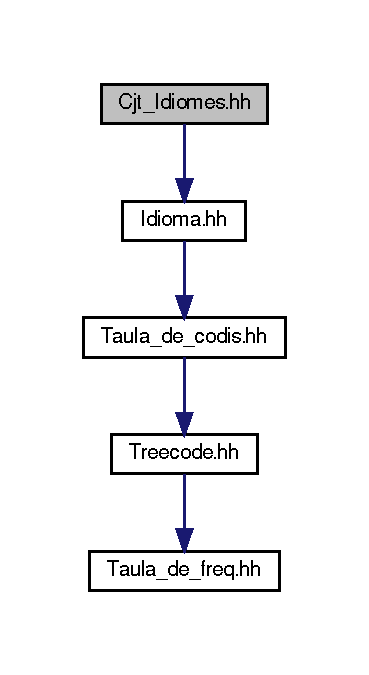
\includegraphics[width=177pt]{_cjt___idiomes_8hh__incl}
\end{center}
\end{figure}
\subsection*{Clases}
\begin{DoxyCompactItemize}
\item 
class \hyperlink{class_cjt___idiomes}{Cjt\+\_\+\+Idiomes}
\begin{DoxyCompactList}\small\item\em Representa un \hyperlink{class_cjt___idiomes}{Cjt\+\_\+\+Idiomes}. \end{DoxyCompactList}\end{DoxyCompactItemize}


\subsection{Descripción detallada}
Especificació de la classe \hyperlink{class_cjt___idiomes}{Cjt\+\_\+\+Idiomes}. 


\hypertarget{_idioma_8hh}{}\section{Referencia del Archivo Idioma.\+hh}
\label{_idioma_8hh}\index{Idioma.\+hh@{Idioma.\+hh}}


Especificació de la classe \hyperlink{class_idioma}{Idioma}.  


Dependencia gráfica adjunta para Idioma.\+hh\+:\nopagebreak
\begin{figure}[H]
\begin{center}
\leavevmode
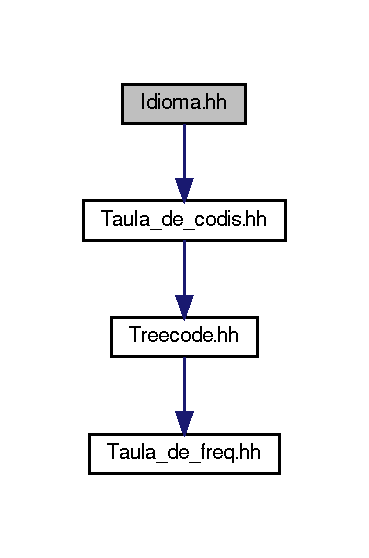
\includegraphics[width=193pt]{_idioma_8hh__incl}
\end{center}
\end{figure}
\subsection*{Clases}
\begin{DoxyCompactItemize}
\item 
class \hyperlink{class_idioma}{Idioma}
\begin{DoxyCompactList}\small\item\em Representa un \hyperlink{class_idioma}{Idioma}. \end{DoxyCompactList}\end{DoxyCompactItemize}


\subsection{Descripción detallada}
Especificació de la classe \hyperlink{class_idioma}{Idioma}. 


\hypertarget{program_8cc}{}\section{Referencia del Archivo program.\+cc}
\label{program_8cc}\index{program.\+cc@{program.\+cc}}


Programa principal per la gestió de codificar i descodificar.  


Dependencia gráfica adjunta para program.\+cc\+:\nopagebreak
\begin{figure}[H]
\begin{center}
\leavevmode
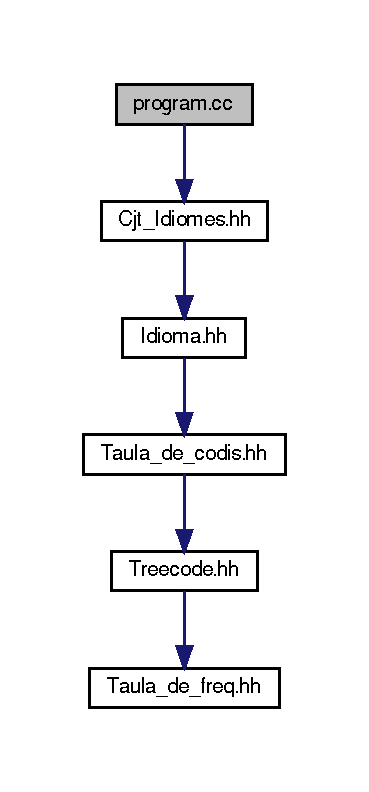
\includegraphics[width=177pt]{program_8cc__incl}
\end{center}
\end{figure}
\subsection*{Funciones}
\begin{DoxyCompactItemize}
\item 
int \hyperlink{program_8cc_ae66f6b31b5ad750f1fe042a706a4e3d4}{main} ()
\end{DoxyCompactItemize}


\subsection{Descripción detallada}
Programa principal per la gestió de codificar i descodificar. 



\subsection{Documentación de las funciones}
\mbox{\Hypertarget{program_8cc_ae66f6b31b5ad750f1fe042a706a4e3d4}\label{program_8cc_ae66f6b31b5ad750f1fe042a706a4e3d4}} 
\index{program.\+cc@{program.\+cc}!main@{main}}
\index{main@{main}!program.\+cc@{program.\+cc}}
\subsubsection{\texorpdfstring{main()}{main()}}
{\footnotesize\ttfamily int main (\begin{DoxyParamCaption}{ }\end{DoxyParamCaption})}



Definición en la línea 21 del archivo program.\+cc.


\begin{DoxyCode}
21            \{
22     
23     \hyperlink{class_cjt___idiomes}{Cjt\_Idiomes} conjunt;
24     conjunt.\hyperlink{class_cjt___idiomes_a27ad0dd99449fffa904e6a757b4388ad}{omplir\_cjt\_idiomes}();
25     
26     \textcolor{keywordtype}{string} op;
27     \textcolor{keywordtype}{string} nomidioma, text;
28     \textcolor{keywordflow}{while}(op != \textcolor{stringliteral}{"fin"})\{
29         
30         \textcolor{keywordflow}{if}(op == \textcolor{stringliteral}{"añadir"} or op == \textcolor{stringliteral}{"modificar"})\{
31             cin >> nomidioma;
32             conjunt.\hyperlink{class_cjt___idiomes_a9e75f643c62886df635403bd3108c1df}{afegir\_modificar\_idioma} (nomidioma);
33         \}
34         
35         \textcolor{keywordflow}{else} \textcolor{keywordflow}{if}(op == \textcolor{stringliteral}{"codifica"})\{
36             cin >> nomidioma >> text;
37             \textcolor{keywordflow}{if} (conjunt.\hyperlink{class_cjt___idiomes_a699b46fae0fb902952cc5cad27604928}{idioma\_esta} (nomidioma, conjunt)) conjunt.
      \hyperlink{class_cjt___idiomes_a745de8e5d29e235cb1e2142d8acaaad9}{codifica} (nomidioma, text);
38         \}
39         
40         \textcolor{keywordflow}{else} \textcolor{keywordflow}{if}(op == \textcolor{stringliteral}{"decodifica"})\{
41             cin >> nomidioma >> text;
42             \textcolor{keywordflow}{if} (conjunt.\hyperlink{class_cjt___idiomes_a699b46fae0fb902952cc5cad27604928}{idioma\_esta} (nomidioma, conjunt)) conjunt.
      \hyperlink{class_cjt___idiomes_ab77062c4c2b311bbc1fc1143073bc036}{decodifica} (nomidioma, text);
43         \}
44         
45         \textcolor{keywordflow}{else} \textcolor{keywordflow}{if}(op == \textcolor{stringliteral}{"tabla\_frec"})\{
46             cin >> nomidioma;
47             \textcolor{keywordflow}{if} (conjunt.\hyperlink{class_cjt___idiomes_a699b46fae0fb902952cc5cad27604928}{idioma\_esta} (nomidioma, conjunt)) conjunt.
      \hyperlink{class_cjt___idiomes_a10390ac35850d05a28d06dbf6a3deb4f}{consultar\_taula\_freq} (nomidioma);
48         \}
49         
50         \textcolor{keywordflow}{else} \textcolor{keywordflow}{if}(op == \textcolor{stringliteral}{"treecode"})\{
51             cin >> nomidioma;
52             \textcolor{keywordflow}{if} (conjunt.\hyperlink{class_cjt___idiomes_a699b46fae0fb902952cc5cad27604928}{idioma\_esta} (nomidioma, conjunt)) conjunt.
      \hyperlink{class_cjt___idiomes_a2bf21a96cdbba804d53a097c42fe3b93}{consultar\_Treecode} (nomidioma);
53         \}
54         
55         \textcolor{keywordflow}{else} \textcolor{keywordflow}{if}(op == \textcolor{stringliteral}{"codigos"})\{
56             cin >> nomidioma;
57             \textcolor{keywordflow}{if} (conjunt.\hyperlink{class_cjt___idiomes_a699b46fae0fb902952cc5cad27604928}{idioma\_esta} (nomidioma, conjunt)) conjunt.
      \hyperlink{class_cjt___idiomes_af8497129cf6b3b094e6f26a0c030c785}{consultar\_taula\_codis} (nomidioma);
58         \}
59         
60         cin >> op;
61     \}
62     
63 \}
\end{DoxyCode}

\hypertarget{_taula__de__codis_8hh}{}\section{Referencia del Archivo Taula\+\_\+de\+\_\+codis.\+hh}
\label{_taula__de__codis_8hh}\index{Taula\+\_\+de\+\_\+codis.\+hh@{Taula\+\_\+de\+\_\+codis.\+hh}}


Especificació de la classe \hyperlink{class_taula__de__codis}{Taula\+\_\+de\+\_\+codis}.  


Dependencia gráfica adjunta para Taula\+\_\+de\+\_\+codis.\+hh\+:\nopagebreak
\begin{figure}[H]
\begin{center}
\leavevmode
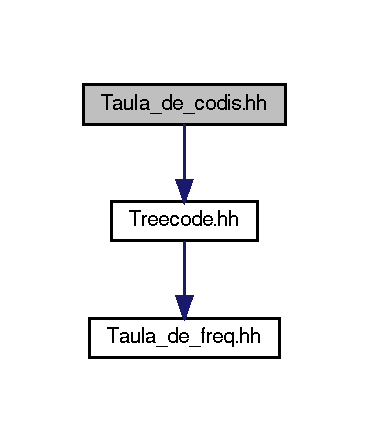
\includegraphics[width=177pt]{_taula__de__codis_8hh__incl}
\end{center}
\end{figure}
\subsection*{Clases}
\begin{DoxyCompactItemize}
\item 
class \hyperlink{class_taula__de__codis}{Taula\+\_\+de\+\_\+codis}
\begin{DoxyCompactList}\small\item\em Representa una \hyperlink{class_taula__de__codis}{Taula\+\_\+de\+\_\+codis}. \end{DoxyCompactList}\end{DoxyCompactItemize}


\subsection{Descripción detallada}
Especificació de la classe \hyperlink{class_taula__de__codis}{Taula\+\_\+de\+\_\+codis}. 


\hypertarget{_taula__de__freq_8hh}{}\section{Referencia del Archivo Taula\+\_\+de\+\_\+freq.\+hh}
\label{_taula__de__freq_8hh}\index{Taula\+\_\+de\+\_\+freq.\+hh@{Taula\+\_\+de\+\_\+freq.\+hh}}


Especificació de la classe \hyperlink{class_taula__de__freq}{Taula\+\_\+de\+\_\+freq}.  


\subsection*{Clases}
\begin{DoxyCompactItemize}
\item 
class \hyperlink{class_taula__de__freq}{Taula\+\_\+de\+\_\+freq}
\begin{DoxyCompactList}\small\item\em Representa una \hyperlink{class_taula__de__freq}{Taula\+\_\+de\+\_\+freq}. \end{DoxyCompactList}\end{DoxyCompactItemize}


\subsection{Descripción detallada}
Especificació de la classe \hyperlink{class_taula__de__freq}{Taula\+\_\+de\+\_\+freq}. 


\hypertarget{_treecode_8hh}{}\section{Referencia del Archivo Treecode.\+hh}
\label{_treecode_8hh}\index{Treecode.\+hh@{Treecode.\+hh}}


Especificació de la classe \hyperlink{class_treecode}{Treecode}.  


Dependencia gráfica adjunta para Treecode.\+hh\+:\nopagebreak
\begin{figure}[H]
\begin{center}
\leavevmode
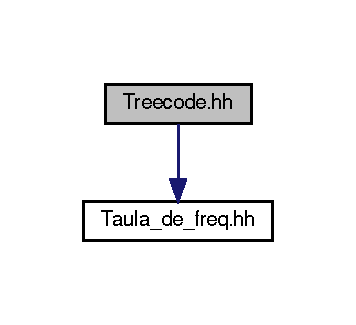
\includegraphics[width=171pt]{_treecode_8hh__incl}
\end{center}
\end{figure}
\subsection*{Clases}
\begin{DoxyCompactItemize}
\item 
class \hyperlink{class_treecode}{Treecode}
\begin{DoxyCompactList}\small\item\em Representa un \hyperlink{class_treecode}{Treecode}. \end{DoxyCompactList}\end{DoxyCompactItemize}


\subsection{Descripción detallada}
Especificació de la classe \hyperlink{class_treecode}{Treecode}. 


%--- End generated contents ---

% Index
\backmatter
\newpage
\phantomsection
\clearemptydoublepage
\addcontentsline{toc}{chapter}{Índice}
\printindex

\end{document}
